\chapter{Introduction} \label{chap:intro}


As a company becomes more reliable on the data it produces to drive its
decisions, a data warehouse is a core component when providing data for analysis
and reporting. The data is extracted from one or more data sources, which can
then be transformed and loaded into the appropriate format for consultation. 

It is also well known that as companies become more data driven, the challenges
associated with dealing with large volumes of data becomes more apparent as
digital solutions start failing to respond, or are unable to respond within
appropriate time constraints. 

For this reason, a distributed architecture that resorts to microservices is a
common and efficient way to tackle the problem as it simplifies scaling based on
the system's needs, nullifies the single point of failure, and increases the
system's resilience, when correctly implemented. 

On the other hand, communication between microservices, when incorrectly
implemented can become the bottleneck of the scalibility of a distributed
solution, as the components can become too coupled and increase the technical
cost of making any changes to the system. This is where message brokers come in.
Instead of having the components communicating with one another directly, the
message broker serves as an intermediary that asynchronously delivers the
information between components as it is requested by the interested parts. When
employing a message broker, two important entities involved in the communication
are data producers (entities that send data to the broker), and data consumers
(entities that request data from the broker). 

\begin{figure}[htb!]
    \centering
    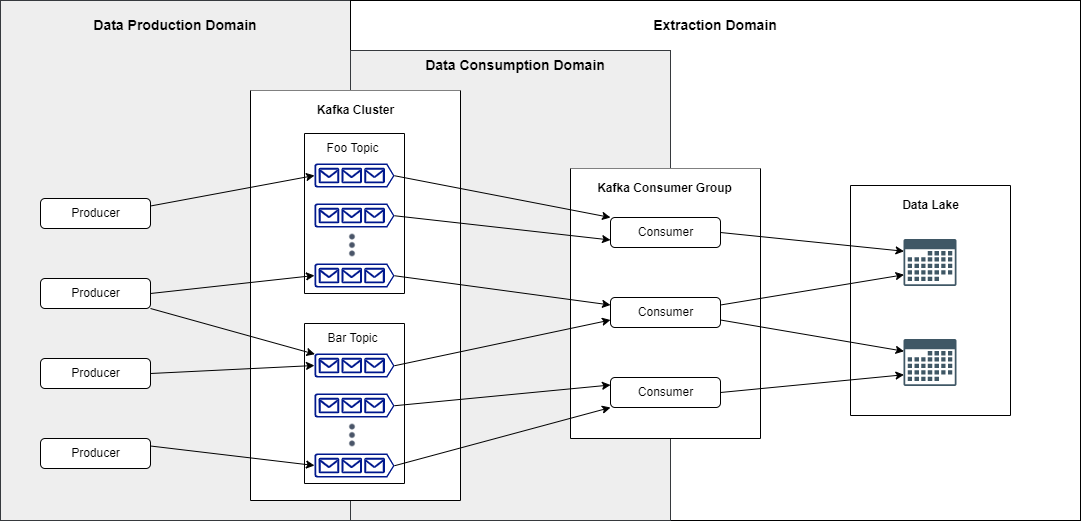
\includegraphics[width=\textwidth]{images/introduction/Context.png}
\caption{
    Data pipeline representing the flow of data since it is appended into one of
    the data sources (Topic), to when it is fetched by a consumer and inserted
    into a Data Lake.
}
\label{fig:problem_context}
\end{figure}


Having used Kafka as the message broker system, a Kafka cluster is made of
topics, which in turn is a unit that is subdivided into several logs, commonly
reffered to as partitions. When a producer sends a record to a specific topic,
it will be appended into one of the topic's partitions, illustrated in the
Data Production Domain in figure \ref{fig:problem_context}. 

A consumer group is a unit composed of multiple consumers, each with the common
task of consuming data from the topics the group is subscribed to. To consume
the data within a topic, each of its partitions have to be assigned a single
consumer belonging to the same group, which is also how Kafka provides
scalability, parallelizing the tasks between the consumers of a group. This
design feature also leads to the fact that a group does not require more
consumers than the number of partitions, as only one consumer in a group can
read data from a given partition.

The problem was proposed by the data engineering team at HUUB (MAERSK), and it
is framed within the scope of the Extraction Domain in figure
\ref{fig:problem_context}, and it consists of being capable to dynamically
determine and manage a group of consumers, that up- and down-scales the
number of instances, and also specifying the tasks (partitions) that are assigned
to each consumer, so as to achieve the required amount of parallelism to
guarantee the number of unread messages by the group does not increase, which is
to say that the rate at which the group is consuming records from each
partition, is bigger or equal to their respective write speed.

Modeling consumers as bins, and partitions as items that have to be assigned a
bin, this problem was modeled as the Bin Packing Problem (BPP), with the
particularity that the items vary in size with time. This occurs because the
partition's size correlates to its current write speed, which fluctuates based
on the current system's load and inevitably implies that a solution for a given
time instant may not hold true in future instants. 

On account of this variation of the BPP, a new solution has to be computed at
each instant that might lead to a partition (item) being assigned to a different
consumer (bin) when compared to the consumer group's previous configuration.
Since two consumers cannot read from the same partition concurrently, the cost
associated to rebalancing a partition is related to the amount of data that is
not being read while the partition is being assigned to another consumer. Hence,
in section \ref{sub:rscore} a new metric is proposed (Rscore) to determine the rebalance
cost for a given iteration. 

Given that it is the first time the Bin Packing Problem is applied in this
context, the existing algorithms do not take the rebalancing cost into account.
For this reason four new algorithms are also proposed in section
\ref{subsub:modified_any_fit} that heuristically solve the Bin Packing Problem
while taking the Rscore into account. 

The algorithm's performance is compared in section \ref{c3subsub:testing}, and
since the algorithms are attempting to solve a multi-objective problem that aims
to minimize both the number of bins required and the rebalance cost for a single
iteration, the pareto front shows that three of the proposed algorithms are a
competitive solution to the problem at hand.

Furthermore, to accomodate the aforementioned theoretical approach to solve the
autoscaling problem, a system comprised of three components delivers an
automated solution to scaling a consumer group, which is presented in chapter
\ref{chap:consumer_group_autoscaler}. Each of the components is unitarily tested throughout
sections \ref{component:Monitor}, \ref{component:consumer} and
\ref{component:controller}. Lastly, an integration test is also presented in
chapter \ref{chap:integration_tests}, aimed to reflect the autoscaler's response
time to the message broker's current load.


